% Created by tikzDevice version 0.6.1 on 2016-06-13 09:53:06
% !TEX encoding = UTF-8 Unicode
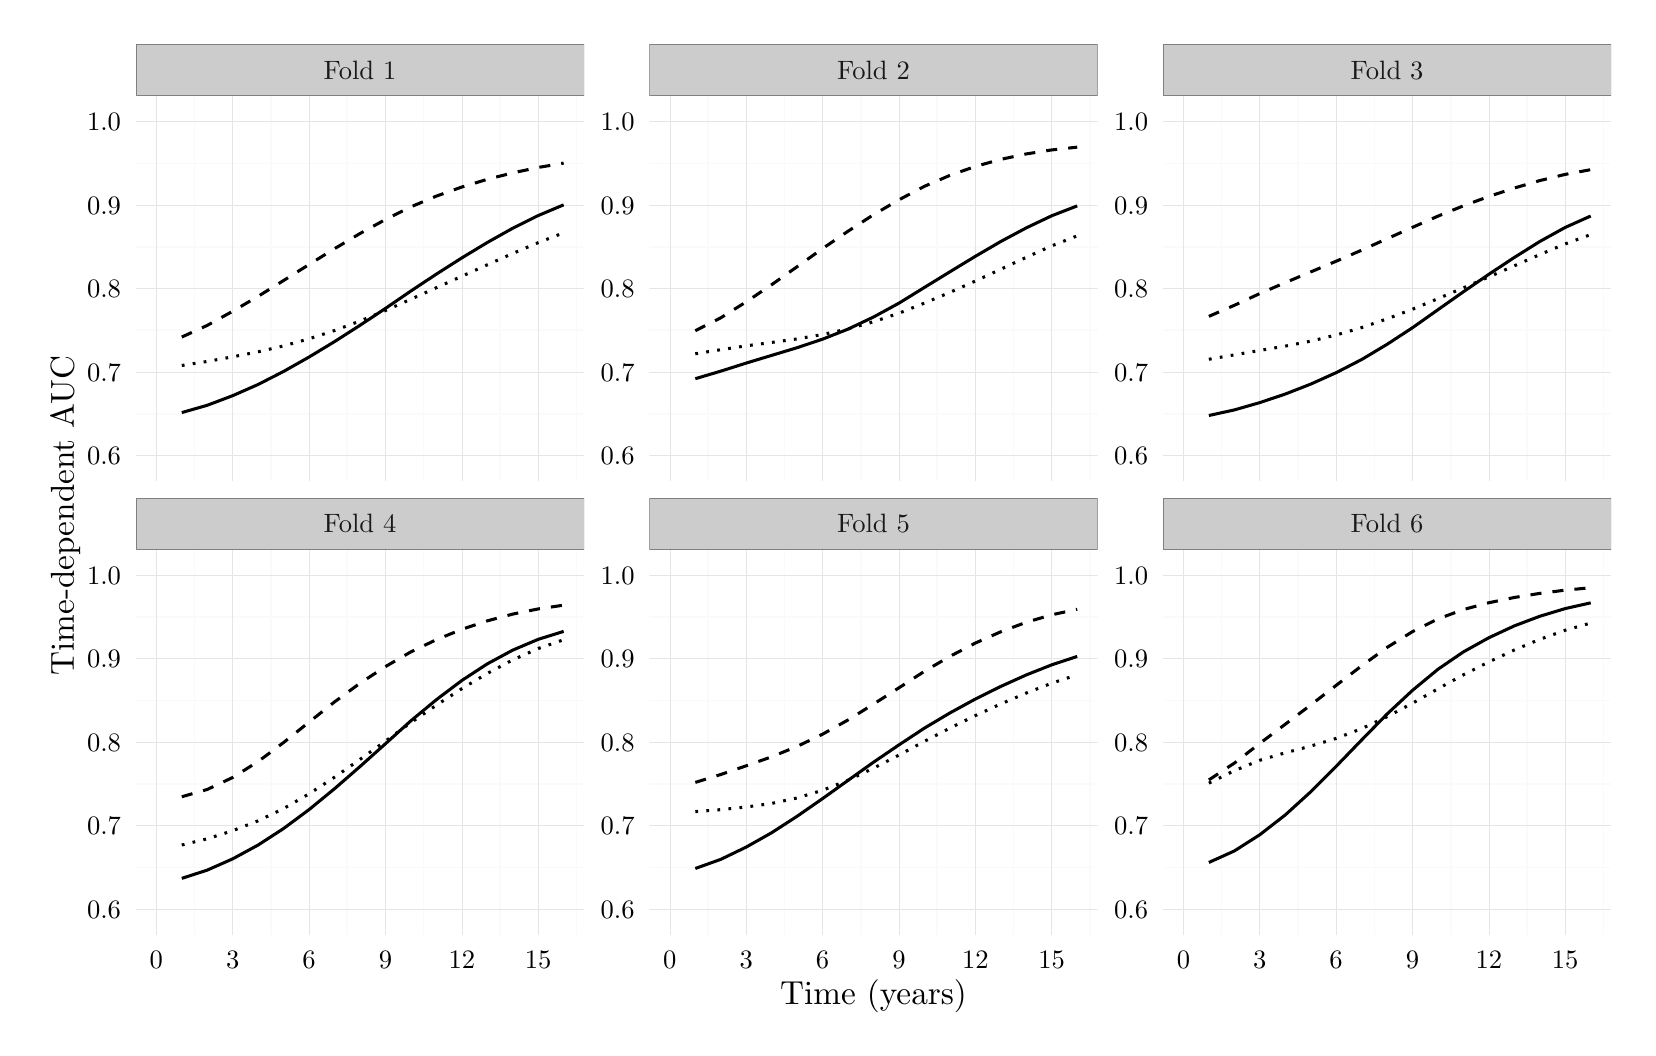
\begin{tikzpicture}[x=1pt,y=1pt]
\definecolor[named]{drawColor}{rgb}{0.00,0.00,0.00}
\definecolor[named]{fillColor}{rgb}{1.00,1.00,1.00}
\fill[color=fillColor,] (0,0) rectangle (578.16,361.35);
\begin{scope}
\path[clip] (  0.00,  0.00) rectangle (578.16,361.35);
\end{scope}
\begin{scope}
\path[clip] (  0.00,  0.00) rectangle (578.16,361.35);
\end{scope}
\begin{scope}
\path[clip] (  0.00,  0.00) rectangle (578.16,361.35);
\end{scope}
\begin{scope}
\path[clip] (  0.00,  0.00) rectangle (578.16,361.35);
\end{scope}
\begin{scope}
\path[clip] (  0.00,  0.00) rectangle (578.16,361.35);
\end{scope}
\begin{scope}
\path[clip] (  0.00,  0.00) rectangle (578.16,361.35);
\end{scope}
\begin{scope}
\path[clip] (  0.00,  0.00) rectangle (578.16,361.35);
\end{scope}
\begin{scope}
\path[clip] (  0.00,  0.00) rectangle (578.16,361.35);
\end{scope}
\begin{scope}
\path[clip] (  0.00,  0.00) rectangle (578.16,361.35);
\end{scope}
\begin{scope}
\path[clip] (  0.00,  0.00) rectangle (578.16,361.35);
\end{scope}
\begin{scope}
\path[clip] (  0.00,  0.00) rectangle (578.16,361.35);
\end{scope}
\begin{scope}
\path[clip] (  0.00,  0.00) rectangle (578.16,361.35);
\end{scope}
\begin{scope}
\path[clip] (  0.00,  0.00) rectangle (578.16,361.35);
\end{scope}
\begin{scope}
\path[clip] (  0.00,  0.00) rectangle (578.16,361.35);
\end{scope}
\begin{scope}
\path[clip] (  0.00,  0.00) rectangle (578.16,361.35);
\end{scope}
\begin{scope}
\path[clip] (  0.00,  0.00) rectangle (578.16,361.35);
\end{scope}
\begin{scope}
\path[clip] (  0.00,  0.00) rectangle (578.16,361.35);
\end{scope}
\begin{scope}
\path[clip] (  0.00,  0.00) rectangle (578.16,361.35);
\end{scope}
\begin{scope}
\path[clip] (  0.00,  0.00) rectangle (578.16,361.35);
\end{scope}
\begin{scope}
\path[clip] (  0.00,  0.00) rectangle (578.16,361.35);
\end{scope}
\begin{scope}
\path[clip] (  0.00,  0.00) rectangle (578.16,361.35);
\end{scope}
\begin{scope}
\path[clip] (  0.00,  0.00) rectangle (578.16,361.35);
\end{scope}
\begin{scope}
\path[clip] (  0.00,  0.00) rectangle (578.16,361.35);
\end{scope}
\begin{scope}
\path[clip] (  0.00,  0.00) rectangle (578.16,361.35);
\end{scope}
\begin{scope}
\path[clip] (  0.00,  0.00) rectangle (578.16,361.35);
\end{scope}
\begin{scope}
\path[clip] (  0.00,  0.00) rectangle (578.16,361.35);
\end{scope}
\begin{scope}
\path[clip] (  0.00,  0.00) rectangle (578.16,361.35);
\end{scope}
\begin{scope}
\path[clip] (  0.00,  0.00) rectangle (578.16,361.35);
\definecolor[named]{drawColor}{rgb}{1.00,1.00,1.00}
\definecolor[named]{fillColor}{rgb}{1.00,1.00,1.00}

\draw[color=drawColor,line width= 0.6pt,line cap=round,line join=round,fill=fillColor,] (  0.00,  0.00) rectangle (578.16,361.35);
\end{scope}
\begin{scope}
\path[clip] (  0.00,  0.00) rectangle (578.16,361.35);
\end{scope}
\begin{scope}
\path[clip] ( 39.13,197.41) rectangle (201.03,336.74);
\definecolor[named]{fillColor}{rgb}{1.00,1.00,1.00}

\draw[fill=fillColor,draw opacity=0.00,] ( 39.13,197.41) rectangle (201.03,336.74);
\definecolor[named]{drawColor}{rgb}{0.98,0.98,0.98}

\draw[color=drawColor,line width= 0.6pt,line join=round,fill opacity=0.00,] ( 39.13,221.84) --
	(201.03,221.84);

\draw[color=drawColor,line width= 0.6pt,line join=round,fill opacity=0.00,] ( 39.13,252.00) --
	(201.03,252.00);

\draw[color=drawColor,line width= 0.6pt,line join=round,fill opacity=0.00,] ( 39.13,282.15) --
	(201.03,282.15);

\draw[color=drawColor,line width= 0.6pt,line join=round,fill opacity=0.00,] ( 39.13,312.31) --
	(201.03,312.31);

\draw[color=drawColor,line width= 0.6pt,line join=round,fill opacity=0.00,] ( 60.29,197.41) --
	( 60.29,336.74);

\draw[color=drawColor,line width= 0.6pt,line join=round,fill opacity=0.00,] ( 87.88,197.41) --
	( 87.88,336.74);

\draw[color=drawColor,line width= 0.6pt,line join=round,fill opacity=0.00,] (115.48,197.41) --
	(115.48,336.74);

\draw[color=drawColor,line width= 0.6pt,line join=round,fill opacity=0.00,] (143.08,197.41) --
	(143.08,336.74);

\draw[color=drawColor,line width= 0.6pt,line join=round,fill opacity=0.00,] (170.67,197.41) --
	(170.67,336.74);

\draw[color=drawColor,line width= 0.6pt,line join=round,fill opacity=0.00,] (198.27,197.41) --
	(198.27,336.74);
\definecolor[named]{drawColor}{rgb}{0.90,0.90,0.90}

\draw[color=drawColor,line width= 0.2pt,line join=round,fill opacity=0.00,] ( 39.13,206.76) --
	(201.03,206.76);

\draw[color=drawColor,line width= 0.2pt,line join=round,fill opacity=0.00,] ( 39.13,236.92) --
	(201.03,236.92);

\draw[color=drawColor,line width= 0.2pt,line join=round,fill opacity=0.00,] ( 39.13,267.08) --
	(201.03,267.08);

\draw[color=drawColor,line width= 0.2pt,line join=round,fill opacity=0.00,] ( 39.13,297.23) --
	(201.03,297.23);

\draw[color=drawColor,line width= 0.2pt,line join=round,fill opacity=0.00,] ( 39.13,327.39) --
	(201.03,327.39);

\draw[color=drawColor,line width= 0.2pt,line join=round,fill opacity=0.00,] ( 46.49,197.41) --
	( 46.49,336.74);

\draw[color=drawColor,line width= 0.2pt,line join=round,fill opacity=0.00,] ( 74.08,197.41) --
	( 74.08,336.74);

\draw[color=drawColor,line width= 0.2pt,line join=round,fill opacity=0.00,] (101.68,197.41) --
	(101.68,336.74);

\draw[color=drawColor,line width= 0.2pt,line join=round,fill opacity=0.00,] (129.28,197.41) --
	(129.28,336.74);

\draw[color=drawColor,line width= 0.2pt,line join=round,fill opacity=0.00,] (156.87,197.41) --
	(156.87,336.74);

\draw[color=drawColor,line width= 0.2pt,line join=round,fill opacity=0.00,] (184.47,197.41) --
	(184.47,336.74);
\definecolor[named]{drawColor}{rgb}{0.00,0.00,0.00}
\definecolor[named]{fillColor}{rgb}{0.00,0.00,0.00}

\draw[color=drawColor,line width= 1.1pt,line join=round,] ( 55.69,222.26) --
	( 64.89,224.90) --
	( 74.08,228.37) --
	( 83.28,232.42) --
	( 92.48,237.13) --
	(101.68,242.33) --
	(110.88,247.90) --
	(120.08,253.79) --
	(129.28,259.90) --
	(138.48,266.20) --
	(147.68,272.29) --
	(156.87,278.15) --
	(166.07,283.71) --
	(175.27,288.87) --
	(184.47,293.45) --
	(193.67,297.33);

\draw[color=drawColor,line width= 1.1pt,dash pattern=on 1pt off 3pt ,line join=round,] ( 55.69,239.28) --
	( 64.89,240.74) --
	( 74.08,242.41) --
	( 83.28,244.22) --
	( 92.48,246.36) --
	(101.68,248.91) --
	(110.88,251.91) --
	(120.08,255.34) --
	(129.28,259.13) --
	(138.48,263.24) --
	(147.68,267.37) --
	(156.87,271.52) --
	(166.07,275.66) --
	(175.27,279.76) --
	(184.47,283.66) --
	(193.67,287.22);

\draw[color=drawColor,line width= 1.1pt,dash pattern=on 4pt off 4pt ,line join=round,] ( 55.69,249.56) --
	( 64.89,253.77) --
	( 74.08,258.88) --
	( 83.28,264.27) --
	( 92.48,269.99) --
	(101.68,275.77) --
	(110.88,281.48) --
	(120.08,286.96) --
	(129.28,292.02) --
	(138.48,296.61) --
	(147.68,300.48) --
	(156.87,303.76) --
	(166.07,306.54) --
	(175.27,308.88) --
	(184.47,310.83) --
	(193.67,312.40);
\end{scope}
\begin{scope}
\path[clip] (  0.00,  0.00) rectangle (578.16,361.35);
\end{scope}
\begin{scope}
\path[clip] (224.69,197.41) rectangle (386.59,336.74);
\definecolor[named]{fillColor}{rgb}{1.00,1.00,1.00}

\draw[fill=fillColor,draw opacity=0.00,] (224.69,197.41) rectangle (386.59,336.74);
\definecolor[named]{drawColor}{rgb}{0.98,0.98,0.98}

\draw[color=drawColor,line width= 0.6pt,line join=round,fill opacity=0.00,] (224.69,221.84) --
	(386.59,221.84);

\draw[color=drawColor,line width= 0.6pt,line join=round,fill opacity=0.00,] (224.69,252.00) --
	(386.59,252.00);

\draw[color=drawColor,line width= 0.6pt,line join=round,fill opacity=0.00,] (224.69,282.15) --
	(386.59,282.15);

\draw[color=drawColor,line width= 0.6pt,line join=round,fill opacity=0.00,] (224.69,312.31) --
	(386.59,312.31);

\draw[color=drawColor,line width= 0.6pt,line join=round,fill opacity=0.00,] (245.85,197.41) --
	(245.85,336.74);

\draw[color=drawColor,line width= 0.6pt,line join=round,fill opacity=0.00,] (273.45,197.41) --
	(273.45,336.74);

\draw[color=drawColor,line width= 0.6pt,line join=round,fill opacity=0.00,] (301.04,197.41) --
	(301.04,336.74);

\draw[color=drawColor,line width= 0.6pt,line join=round,fill opacity=0.00,] (328.64,197.41) --
	(328.64,336.74);

\draw[color=drawColor,line width= 0.6pt,line join=round,fill opacity=0.00,] (356.24,197.41) --
	(356.24,336.74);

\draw[color=drawColor,line width= 0.6pt,line join=round,fill opacity=0.00,] (383.84,197.41) --
	(383.84,336.74);
\definecolor[named]{drawColor}{rgb}{0.90,0.90,0.90}

\draw[color=drawColor,line width= 0.2pt,line join=round,fill opacity=0.00,] (224.69,206.76) --
	(386.59,206.76);

\draw[color=drawColor,line width= 0.2pt,line join=round,fill opacity=0.00,] (224.69,236.92) --
	(386.59,236.92);

\draw[color=drawColor,line width= 0.2pt,line join=round,fill opacity=0.00,] (224.69,267.08) --
	(386.59,267.08);

\draw[color=drawColor,line width= 0.2pt,line join=round,fill opacity=0.00,] (224.69,297.23) --
	(386.59,297.23);

\draw[color=drawColor,line width= 0.2pt,line join=round,fill opacity=0.00,] (224.69,327.39) --
	(386.59,327.39);

\draw[color=drawColor,line width= 0.2pt,line join=round,fill opacity=0.00,] (232.05,197.41) --
	(232.05,336.74);

\draw[color=drawColor,line width= 0.2pt,line join=round,fill opacity=0.00,] (259.65,197.41) --
	(259.65,336.74);

\draw[color=drawColor,line width= 0.2pt,line join=round,fill opacity=0.00,] (287.25,197.41) --
	(287.25,336.74);

\draw[color=drawColor,line width= 0.2pt,line join=round,fill opacity=0.00,] (314.84,197.41) --
	(314.84,336.74);

\draw[color=drawColor,line width= 0.2pt,line join=round,fill opacity=0.00,] (342.44,197.41) --
	(342.44,336.74);

\draw[color=drawColor,line width= 0.2pt,line join=round,fill opacity=0.00,] (370.04,197.41) --
	(370.04,336.74);
\definecolor[named]{drawColor}{rgb}{0.00,0.00,0.00}
\definecolor[named]{fillColor}{rgb}{0.00,0.00,0.00}

\draw[color=drawColor,line width= 1.1pt,line join=round,] (241.25,234.50) --
	(250.45,237.23) --
	(259.65,240.15) --
	(268.85,242.93) --
	(278.05,245.71) --
	(287.25,248.80) --
	(296.45,252.42) --
	(305.64,256.79) --
	(314.84,261.80) --
	(324.04,267.48) --
	(333.24,273.13) --
	(342.44,278.72) --
	(351.64,284.09) --
	(360.84,289.00) --
	(370.04,293.38) --
	(379.24,296.94);

\draw[color=drawColor,line width= 1.1pt,dash pattern=on 1pt off 3pt ,line join=round,] (241.25,243.51) --
	(250.45,244.98) --
	(259.65,246.38) --
	(268.85,247.61) --
	(278.05,248.89) --
	(287.25,250.47) --
	(296.45,252.50) --
	(305.64,255.08) --
	(314.84,258.17) --
	(324.04,261.82) --
	(333.24,265.68) --
	(342.44,269.79) --
	(351.64,274.07) --
	(360.84,278.36) --
	(370.04,282.51) --
	(379.24,286.11);

\draw[color=drawColor,line width= 1.1pt,dash pattern=on 4pt off 4pt ,line join=round,] (241.25,251.85) --
	(250.45,256.51) --
	(259.65,262.28) --
	(268.85,268.48) --
	(278.05,274.98) --
	(287.25,281.54) --
	(296.45,287.81) --
	(305.64,293.76) --
	(314.84,299.15) --
	(324.04,304.02) --
	(333.24,307.97) --
	(342.44,311.20) --
	(351.64,313.77) --
	(360.84,315.72) --
	(370.04,317.17) --
	(379.24,318.17);
\end{scope}
\begin{scope}
\path[clip] (  0.00,  0.00) rectangle (578.16,361.35);
\end{scope}
\begin{scope}
\path[clip] (410.26,197.41) rectangle (572.16,336.74);
\definecolor[named]{fillColor}{rgb}{1.00,1.00,1.00}

\draw[fill=fillColor,draw opacity=0.00,] (410.26,197.41) rectangle (572.16,336.74);
\definecolor[named]{drawColor}{rgb}{0.98,0.98,0.98}

\draw[color=drawColor,line width= 0.6pt,line join=round,fill opacity=0.00,] (410.26,221.84) --
	(572.16,221.84);

\draw[color=drawColor,line width= 0.6pt,line join=round,fill opacity=0.00,] (410.26,252.00) --
	(572.16,252.00);

\draw[color=drawColor,line width= 0.6pt,line join=round,fill opacity=0.00,] (410.26,282.15) --
	(572.16,282.15);

\draw[color=drawColor,line width= 0.6pt,line join=round,fill opacity=0.00,] (410.26,312.31) --
	(572.16,312.31);

\draw[color=drawColor,line width= 0.6pt,line join=round,fill opacity=0.00,] (431.42,197.41) --
	(431.42,336.74);

\draw[color=drawColor,line width= 0.6pt,line join=round,fill opacity=0.00,] (459.01,197.41) --
	(459.01,336.74);

\draw[color=drawColor,line width= 0.6pt,line join=round,fill opacity=0.00,] (486.61,197.41) --
	(486.61,336.74);

\draw[color=drawColor,line width= 0.6pt,line join=round,fill opacity=0.00,] (514.21,197.41) --
	(514.21,336.74);

\draw[color=drawColor,line width= 0.6pt,line join=round,fill opacity=0.00,] (541.80,197.41) --
	(541.80,336.74);

\draw[color=drawColor,line width= 0.6pt,line join=round,fill opacity=0.00,] (569.40,197.41) --
	(569.40,336.74);
\definecolor[named]{drawColor}{rgb}{0.90,0.90,0.90}

\draw[color=drawColor,line width= 0.2pt,line join=round,fill opacity=0.00,] (410.26,206.76) --
	(572.16,206.76);

\draw[color=drawColor,line width= 0.2pt,line join=round,fill opacity=0.00,] (410.26,236.92) --
	(572.16,236.92);

\draw[color=drawColor,line width= 0.2pt,line join=round,fill opacity=0.00,] (410.26,267.08) --
	(572.16,267.08);

\draw[color=drawColor,line width= 0.2pt,line join=round,fill opacity=0.00,] (410.26,297.23) --
	(572.16,297.23);

\draw[color=drawColor,line width= 0.2pt,line join=round,fill opacity=0.00,] (410.26,327.39) --
	(572.16,327.39);

\draw[color=drawColor,line width= 0.2pt,line join=round,fill opacity=0.00,] (417.62,197.41) --
	(417.62,336.74);

\draw[color=drawColor,line width= 0.2pt,line join=round,fill opacity=0.00,] (445.21,197.41) --
	(445.21,336.74);

\draw[color=drawColor,line width= 0.2pt,line join=round,fill opacity=0.00,] (472.81,197.41) --
	(472.81,336.74);

\draw[color=drawColor,line width= 0.2pt,line join=round,fill opacity=0.00,] (500.41,197.41) --
	(500.41,336.74);

\draw[color=drawColor,line width= 0.2pt,line join=round,fill opacity=0.00,] (528.01,197.41) --
	(528.01,336.74);

\draw[color=drawColor,line width= 0.2pt,line join=round,fill opacity=0.00,] (555.60,197.41) --
	(555.60,336.74);
\definecolor[named]{drawColor}{rgb}{0.00,0.00,0.00}
\definecolor[named]{fillColor}{rgb}{0.00,0.00,0.00}

\draw[color=drawColor,line width= 1.1pt,line join=round,] (426.82,221.20) --
	(436.02,223.22) --
	(445.21,225.86) --
	(454.41,228.95) --
	(463.61,232.54) --
	(472.81,236.68) --
	(482.01,241.42) --
	(491.21,246.92) --
	(500.41,252.93) --
	(509.61,259.44) --
	(518.81,265.92) --
	(528.01,272.24) --
	(537.20,278.32) --
	(546.40,284.08) --
	(555.60,289.17) --
	(564.80,293.29);

\draw[color=drawColor,line width= 1.1pt,dash pattern=on 1pt off 3pt ,line join=round,] (426.82,241.53) --
	(436.02,243.12) --
	(445.21,244.71) --
	(454.41,246.27) --
	(463.61,248.07) --
	(472.81,250.29) --
	(482.01,252.97) --
	(491.21,256.13) --
	(500.41,259.61) --
	(509.61,263.44) --
	(518.81,267.34) --
	(528.01,271.29) --
	(537.20,275.30) --
	(546.40,279.35) --
	(555.60,283.21) --
	(564.80,286.58);

\draw[color=drawColor,line width= 1.1pt,dash pattern=on 4pt off 4pt ,line join=round,] (426.82,257.03) --
	(436.02,261.02) --
	(445.21,265.26) --
	(454.41,269.21) --
	(463.61,273.08) --
	(472.81,276.95) --
	(482.01,280.94) --
	(491.21,285.09) --
	(500.41,289.19) --
	(509.61,293.25) --
	(518.81,296.98) --
	(528.01,300.36) --
	(537.20,303.40) --
	(546.40,306.09) --
	(555.60,308.33) --
	(564.80,310.04);
\end{scope}
\begin{scope}
\path[clip] (  0.00,  0.00) rectangle (578.16,361.35);
\end{scope}
\begin{scope}
\path[clip] ( 39.13, 33.48) rectangle (201.03,172.80);
\definecolor[named]{fillColor}{rgb}{1.00,1.00,1.00}

\draw[fill=fillColor,draw opacity=0.00,] ( 39.13, 33.48) rectangle (201.03,172.80);
\definecolor[named]{drawColor}{rgb}{0.98,0.98,0.98}

\draw[color=drawColor,line width= 0.6pt,line join=round,fill opacity=0.00,] ( 39.13, 57.90) --
	(201.03, 57.90);

\draw[color=drawColor,line width= 0.6pt,line join=round,fill opacity=0.00,] ( 39.13, 88.06) --
	(201.03, 88.06);

\draw[color=drawColor,line width= 0.6pt,line join=round,fill opacity=0.00,] ( 39.13,118.22) --
	(201.03,118.22);

\draw[color=drawColor,line width= 0.6pt,line join=round,fill opacity=0.00,] ( 39.13,148.37) --
	(201.03,148.37);

\draw[color=drawColor,line width= 0.6pt,line join=round,fill opacity=0.00,] ( 60.29, 33.48) --
	( 60.29,172.80);

\draw[color=drawColor,line width= 0.6pt,line join=round,fill opacity=0.00,] ( 87.88, 33.48) --
	( 87.88,172.80);

\draw[color=drawColor,line width= 0.6pt,line join=round,fill opacity=0.00,] (115.48, 33.48) --
	(115.48,172.80);

\draw[color=drawColor,line width= 0.6pt,line join=round,fill opacity=0.00,] (143.08, 33.48) --
	(143.08,172.80);

\draw[color=drawColor,line width= 0.6pt,line join=round,fill opacity=0.00,] (170.67, 33.48) --
	(170.67,172.80);

\draw[color=drawColor,line width= 0.6pt,line join=round,fill opacity=0.00,] (198.27, 33.48) --
	(198.27,172.80);
\definecolor[named]{drawColor}{rgb}{0.90,0.90,0.90}

\draw[color=drawColor,line width= 0.2pt,line join=round,fill opacity=0.00,] ( 39.13, 42.83) --
	(201.03, 42.83);

\draw[color=drawColor,line width= 0.2pt,line join=round,fill opacity=0.00,] ( 39.13, 72.98) --
	(201.03, 72.98);

\draw[color=drawColor,line width= 0.2pt,line join=round,fill opacity=0.00,] ( 39.13,103.14) --
	(201.03,103.14);

\draw[color=drawColor,line width= 0.2pt,line join=round,fill opacity=0.00,] ( 39.13,133.30) --
	(201.03,133.30);

\draw[color=drawColor,line width= 0.2pt,line join=round,fill opacity=0.00,] ( 39.13,163.45) --
	(201.03,163.45);

\draw[color=drawColor,line width= 0.2pt,line join=round,fill opacity=0.00,] ( 46.49, 33.48) --
	( 46.49,172.80);

\draw[color=drawColor,line width= 0.2pt,line join=round,fill opacity=0.00,] ( 74.08, 33.48) --
	( 74.08,172.80);

\draw[color=drawColor,line width= 0.2pt,line join=round,fill opacity=0.00,] (101.68, 33.48) --
	(101.68,172.80);

\draw[color=drawColor,line width= 0.2pt,line join=round,fill opacity=0.00,] (129.28, 33.48) --
	(129.28,172.80);

\draw[color=drawColor,line width= 0.2pt,line join=round,fill opacity=0.00,] (156.87, 33.48) --
	(156.87,172.80);

\draw[color=drawColor,line width= 0.2pt,line join=round,fill opacity=0.00,] (184.47, 33.48) --
	(184.47,172.80);
\definecolor[named]{drawColor}{rgb}{0.00,0.00,0.00}
\definecolor[named]{fillColor}{rgb}{0.00,0.00,0.00}

\draw[color=drawColor,line width= 1.1pt,line join=round,] ( 55.69, 53.95) --
	( 64.89, 56.93) --
	( 74.08, 61.00) --
	( 83.28, 66.00) --
	( 92.48, 71.97) --
	(101.68, 78.80) --
	(110.88, 86.34) --
	(120.08, 94.35) --
	(129.28,102.59) --
	(138.48,110.90) --
	(147.68,118.51) --
	(156.87,125.45) --
	(166.07,131.45) --
	(175.27,136.42) --
	(184.47,140.32) --
	(193.67,143.19);

\draw[color=drawColor,line width= 1.1pt,dash pattern=on 1pt off 3pt ,line join=round,] ( 55.69, 66.01) --
	( 64.89, 68.25) --
	( 74.08, 71.17) --
	( 83.28, 74.75) --
	( 92.48, 79.18) --
	(101.68, 84.49) --
	(110.88, 90.50) --
	(120.08, 96.93) --
	(129.28,103.54) --
	(138.48,110.25) --
	(147.68,116.52) --
	(156.87,122.50) --
	(166.07,127.99) --
	(175.27,132.89) --
	(184.47,137.00) --
	(193.67,140.18);

\draw[color=drawColor,line width= 1.1pt,dash pattern=on 4pt off 4pt ,line join=round,] ( 55.69, 83.44) --
	( 64.89, 86.08) --
	( 74.08, 90.40) --
	( 83.28, 96.17) --
	( 92.48,103.04) --
	(101.68,110.41) --
	(110.88,117.71) --
	(120.08,124.46) --
	(129.28,130.47) --
	(138.48,135.80) --
	(147.68,140.20) --
	(156.87,143.94) --
	(166.07,147.00) --
	(175.27,149.44) --
	(184.47,151.31) --
	(193.67,152.67);
\end{scope}
\begin{scope}
\path[clip] (  0.00,  0.00) rectangle (578.16,361.35);
\end{scope}
\begin{scope}
\path[clip] (224.69, 33.48) rectangle (386.59,172.80);
\definecolor[named]{fillColor}{rgb}{1.00,1.00,1.00}

\draw[fill=fillColor,draw opacity=0.00,] (224.69, 33.48) rectangle (386.59,172.80);
\definecolor[named]{drawColor}{rgb}{0.98,0.98,0.98}

\draw[color=drawColor,line width= 0.6pt,line join=round,fill opacity=0.00,] (224.69, 57.90) --
	(386.59, 57.90);

\draw[color=drawColor,line width= 0.6pt,line join=round,fill opacity=0.00,] (224.69, 88.06) --
	(386.59, 88.06);

\draw[color=drawColor,line width= 0.6pt,line join=round,fill opacity=0.00,] (224.69,118.22) --
	(386.59,118.22);

\draw[color=drawColor,line width= 0.6pt,line join=round,fill opacity=0.00,] (224.69,148.37) --
	(386.59,148.37);

\draw[color=drawColor,line width= 0.6pt,line join=round,fill opacity=0.00,] (245.85, 33.48) --
	(245.85,172.80);

\draw[color=drawColor,line width= 0.6pt,line join=round,fill opacity=0.00,] (273.45, 33.48) --
	(273.45,172.80);

\draw[color=drawColor,line width= 0.6pt,line join=round,fill opacity=0.00,] (301.04, 33.48) --
	(301.04,172.80);

\draw[color=drawColor,line width= 0.6pt,line join=round,fill opacity=0.00,] (328.64, 33.48) --
	(328.64,172.80);

\draw[color=drawColor,line width= 0.6pt,line join=round,fill opacity=0.00,] (356.24, 33.48) --
	(356.24,172.80);

\draw[color=drawColor,line width= 0.6pt,line join=round,fill opacity=0.00,] (383.84, 33.48) --
	(383.84,172.80);
\definecolor[named]{drawColor}{rgb}{0.90,0.90,0.90}

\draw[color=drawColor,line width= 0.2pt,line join=round,fill opacity=0.00,] (224.69, 42.83) --
	(386.59, 42.83);

\draw[color=drawColor,line width= 0.2pt,line join=round,fill opacity=0.00,] (224.69, 72.98) --
	(386.59, 72.98);

\draw[color=drawColor,line width= 0.2pt,line join=round,fill opacity=0.00,] (224.69,103.14) --
	(386.59,103.14);

\draw[color=drawColor,line width= 0.2pt,line join=round,fill opacity=0.00,] (224.69,133.30) --
	(386.59,133.30);

\draw[color=drawColor,line width= 0.2pt,line join=round,fill opacity=0.00,] (224.69,163.45) --
	(386.59,163.45);

\draw[color=drawColor,line width= 0.2pt,line join=round,fill opacity=0.00,] (232.05, 33.48) --
	(232.05,172.80);

\draw[color=drawColor,line width= 0.2pt,line join=round,fill opacity=0.00,] (259.65, 33.48) --
	(259.65,172.80);

\draw[color=drawColor,line width= 0.2pt,line join=round,fill opacity=0.00,] (287.25, 33.48) --
	(287.25,172.80);

\draw[color=drawColor,line width= 0.2pt,line join=round,fill opacity=0.00,] (314.84, 33.48) --
	(314.84,172.80);

\draw[color=drawColor,line width= 0.2pt,line join=round,fill opacity=0.00,] (342.44, 33.48) --
	(342.44,172.80);

\draw[color=drawColor,line width= 0.2pt,line join=round,fill opacity=0.00,] (370.04, 33.48) --
	(370.04,172.80);
\definecolor[named]{drawColor}{rgb}{0.00,0.00,0.00}
\definecolor[named]{fillColor}{rgb}{0.00,0.00,0.00}

\draw[color=drawColor,line width= 1.1pt,line join=round,] (241.25, 57.52) --
	(250.45, 60.82) --
	(259.65, 65.26) --
	(268.85, 70.45) --
	(278.05, 76.40) --
	(287.25, 82.79) --
	(296.45, 89.37) --
	(305.64, 95.92) --
	(314.84,102.18) --
	(324.04,108.24) --
	(333.24,113.72) --
	(342.44,118.75) --
	(351.64,123.31) --
	(360.84,127.46) --
	(370.04,131.11) --
	(379.24,134.14);

\draw[color=drawColor,line width= 1.1pt,dash pattern=on 1pt off 3pt ,line join=round,] (241.25, 78.07) --
	(250.45, 78.79) --
	(259.65, 79.74) --
	(268.85, 81.03) --
	(278.05, 83.00) --
	(287.25, 85.79) --
	(296.45, 89.43) --
	(305.64, 93.76) --
	(314.84, 98.48) --
	(324.04,103.47) --
	(333.24,108.24) --
	(342.44,112.77) --
	(351.64,116.98) --
	(360.84,120.91) --
	(370.04,124.47) --
	(379.24,127.51);

\draw[color=drawColor,line width= 1.1pt,dash pattern=on 4pt off 4pt ,line join=round,] (241.25, 88.63) --
	(250.45, 91.48) --
	(259.65, 94.63) --
	(268.85, 97.88) --
	(278.05,101.64) --
	(287.25,106.06) --
	(296.45,111.20) --
	(305.64,116.92) --
	(314.84,122.81) --
	(324.04,128.77) --
	(333.24,134.17) --
	(342.44,138.97) --
	(351.64,143.06) --
	(360.84,146.49) --
	(370.04,149.19) --
	(379.24,151.18);
\end{scope}
\begin{scope}
\path[clip] (  0.00,  0.00) rectangle (578.16,361.35);
\end{scope}
\begin{scope}
\path[clip] (410.26, 33.48) rectangle (572.16,172.80);
\definecolor[named]{fillColor}{rgb}{1.00,1.00,1.00}

\draw[fill=fillColor,draw opacity=0.00,] (410.26, 33.48) rectangle (572.16,172.80);
\definecolor[named]{drawColor}{rgb}{0.98,0.98,0.98}

\draw[color=drawColor,line width= 0.6pt,line join=round,fill opacity=0.00,] (410.26, 57.90) --
	(572.16, 57.90);

\draw[color=drawColor,line width= 0.6pt,line join=round,fill opacity=0.00,] (410.26, 88.06) --
	(572.16, 88.06);

\draw[color=drawColor,line width= 0.6pt,line join=round,fill opacity=0.00,] (410.26,118.22) --
	(572.16,118.22);

\draw[color=drawColor,line width= 0.6pt,line join=round,fill opacity=0.00,] (410.26,148.37) --
	(572.16,148.37);

\draw[color=drawColor,line width= 0.6pt,line join=round,fill opacity=0.00,] (431.42, 33.48) --
	(431.42,172.80);

\draw[color=drawColor,line width= 0.6pt,line join=round,fill opacity=0.00,] (459.01, 33.48) --
	(459.01,172.80);

\draw[color=drawColor,line width= 0.6pt,line join=round,fill opacity=0.00,] (486.61, 33.48) --
	(486.61,172.80);

\draw[color=drawColor,line width= 0.6pt,line join=round,fill opacity=0.00,] (514.21, 33.48) --
	(514.21,172.80);

\draw[color=drawColor,line width= 0.6pt,line join=round,fill opacity=0.00,] (541.80, 33.48) --
	(541.80,172.80);

\draw[color=drawColor,line width= 0.6pt,line join=round,fill opacity=0.00,] (569.40, 33.48) --
	(569.40,172.80);
\definecolor[named]{drawColor}{rgb}{0.90,0.90,0.90}

\draw[color=drawColor,line width= 0.2pt,line join=round,fill opacity=0.00,] (410.26, 42.83) --
	(572.16, 42.83);

\draw[color=drawColor,line width= 0.2pt,line join=round,fill opacity=0.00,] (410.26, 72.98) --
	(572.16, 72.98);

\draw[color=drawColor,line width= 0.2pt,line join=round,fill opacity=0.00,] (410.26,103.14) --
	(572.16,103.14);

\draw[color=drawColor,line width= 0.2pt,line join=round,fill opacity=0.00,] (410.26,133.30) --
	(572.16,133.30);

\draw[color=drawColor,line width= 0.2pt,line join=round,fill opacity=0.00,] (410.26,163.45) --
	(572.16,163.45);

\draw[color=drawColor,line width= 0.2pt,line join=round,fill opacity=0.00,] (417.62, 33.48) --
	(417.62,172.80);

\draw[color=drawColor,line width= 0.2pt,line join=round,fill opacity=0.00,] (445.21, 33.48) --
	(445.21,172.80);

\draw[color=drawColor,line width= 0.2pt,line join=round,fill opacity=0.00,] (472.81, 33.48) --
	(472.81,172.80);

\draw[color=drawColor,line width= 0.2pt,line join=round,fill opacity=0.00,] (500.41, 33.48) --
	(500.41,172.80);

\draw[color=drawColor,line width= 0.2pt,line join=round,fill opacity=0.00,] (528.01, 33.48) --
	(528.01,172.80);

\draw[color=drawColor,line width= 0.2pt,line join=round,fill opacity=0.00,] (555.60, 33.48) --
	(555.60,172.80);
\definecolor[named]{drawColor}{rgb}{0.00,0.00,0.00}
\definecolor[named]{fillColor}{rgb}{0.00,0.00,0.00}

\draw[color=drawColor,line width= 1.1pt,line join=round,] (426.82, 59.70) --
	(436.02, 63.85) --
	(445.21, 69.71) --
	(454.41, 76.85) --
	(463.61, 85.22) --
	(472.81, 94.43) --
	(482.01,103.94) --
	(491.21,113.33) --
	(500.41,121.90) --
	(509.61,129.51) --
	(518.81,135.80) --
	(528.01,140.91) --
	(537.20,145.19) --
	(546.40,148.66) --
	(555.60,151.44) --
	(564.80,153.51);

\draw[color=drawColor,line width= 1.1pt,dash pattern=on 1pt off 3pt ,line join=round,] (426.82, 88.35) --
	(436.02, 92.86) --
	(445.21, 96.62) --
	(454.41, 99.32) --
	(463.61,101.74) --
	(472.81,104.53) --
	(482.01,108.05) --
	(491.21,112.37) --
	(500.41,117.24) --
	(509.61,122.46) --
	(518.81,127.51) --
	(528.01,132.16) --
	(537.20,136.48) --
	(546.40,140.32) --
	(555.60,143.61) --
	(564.80,146.21);

\draw[color=drawColor,line width= 1.1pt,dash pattern=on 4pt off 4pt ,line join=round,] (426.82, 89.53) --
	(436.02, 95.59) --
	(445.21,102.70) --
	(454.41,109.63) --
	(463.61,116.60) --
	(472.81,123.68) --
	(482.01,130.73) --
	(491.21,137.40) --
	(500.41,143.11) --
	(509.61,147.71) --
	(518.81,151.09) --
	(528.01,153.55) --
	(537.20,155.45) --
	(546.40,156.93) --
	(555.60,158.10) --
	(564.80,158.97);
\end{scope}
\begin{scope}
\path[clip] (  0.00,  0.00) rectangle (578.16,361.35);
\end{scope}
\begin{scope}
\path[clip] (  0.00,  0.00) rectangle (578.16,361.35);
\end{scope}
\begin{scope}
\path[clip] ( 39.13,336.74) rectangle (201.03,355.35);
\definecolor[named]{drawColor}{rgb}{0.50,0.50,0.50}
\definecolor[named]{fillColor}{rgb}{0.80,0.80,0.80}

\draw[color=drawColor,line width= 0.2pt,line cap=round,line join=round,fill=fillColor,] ( 39.13,336.74) rectangle (201.03,355.35);
\definecolor[named]{drawColor}{rgb}{0.10,0.10,0.10}

\node[color=drawColor,anchor=base,inner sep=0pt, outer sep=0pt, scale=  0.96] at (120.08,342.74) {Fold 1%
};
\end{scope}
\begin{scope}
\path[clip] ( 39.13,336.74) rectangle (201.03,355.35);
\end{scope}
\begin{scope}
\path[clip] (  0.00,  0.00) rectangle (578.16,361.35);
\end{scope}
\begin{scope}
\path[clip] (  0.00,  0.00) rectangle (578.16,361.35);
\end{scope}
\begin{scope}
\path[clip] (  0.00,  0.00) rectangle (578.16,361.35);
\end{scope}
\begin{scope}
\path[clip] (224.69,336.74) rectangle (386.59,355.35);
\definecolor[named]{drawColor}{rgb}{0.50,0.50,0.50}
\definecolor[named]{fillColor}{rgb}{0.80,0.80,0.80}

\draw[color=drawColor,line width= 0.2pt,line cap=round,line join=round,fill=fillColor,] (224.69,336.74) rectangle (386.59,355.35);
\definecolor[named]{drawColor}{rgb}{0.10,0.10,0.10}

\node[color=drawColor,anchor=base,inner sep=0pt, outer sep=0pt, scale=  0.96] at (305.64,342.74) {Fold 2%
};
\end{scope}
\begin{scope}
\path[clip] (224.69,336.74) rectangle (386.59,355.35);
\end{scope}
\begin{scope}
\path[clip] (  0.00,  0.00) rectangle (578.16,361.35);
\end{scope}
\begin{scope}
\path[clip] (  0.00,  0.00) rectangle (578.16,361.35);
\end{scope}
\begin{scope}
\path[clip] (  0.00,  0.00) rectangle (578.16,361.35);
\end{scope}
\begin{scope}
\path[clip] (410.26,336.74) rectangle (572.16,355.35);
\definecolor[named]{drawColor}{rgb}{0.50,0.50,0.50}
\definecolor[named]{fillColor}{rgb}{0.80,0.80,0.80}

\draw[color=drawColor,line width= 0.2pt,line cap=round,line join=round,fill=fillColor,] (410.26,336.74) rectangle (572.16,355.35);
\definecolor[named]{drawColor}{rgb}{0.10,0.10,0.10}

\node[color=drawColor,anchor=base,inner sep=0pt, outer sep=0pt, scale=  0.96] at (491.21,342.74) {Fold 3%
};
\end{scope}
\begin{scope}
\path[clip] (410.26,336.74) rectangle (572.16,355.35);
\end{scope}
\begin{scope}
\path[clip] (  0.00,  0.00) rectangle (578.16,361.35);
\end{scope}
\begin{scope}
\path[clip] (  0.00,  0.00) rectangle (578.16,361.35);
\end{scope}
\begin{scope}
\path[clip] (  0.00,  0.00) rectangle (578.16,361.35);
\end{scope}
\begin{scope}
\path[clip] ( 39.13,172.80) rectangle (201.03,191.41);
\definecolor[named]{drawColor}{rgb}{0.50,0.50,0.50}
\definecolor[named]{fillColor}{rgb}{0.80,0.80,0.80}

\draw[color=drawColor,line width= 0.2pt,line cap=round,line join=round,fill=fillColor,] ( 39.13,172.80) rectangle (201.03,191.41);
\definecolor[named]{drawColor}{rgb}{0.10,0.10,0.10}

\node[color=drawColor,anchor=base,inner sep=0pt, outer sep=0pt, scale=  0.96] at (120.08,178.80) {Fold 4%
};
\end{scope}
\begin{scope}
\path[clip] ( 39.13,172.80) rectangle (201.03,191.41);
\end{scope}
\begin{scope}
\path[clip] (  0.00,  0.00) rectangle (578.16,361.35);
\end{scope}
\begin{scope}
\path[clip] (  0.00,  0.00) rectangle (578.16,361.35);
\end{scope}
\begin{scope}
\path[clip] (  0.00,  0.00) rectangle (578.16,361.35);
\end{scope}
\begin{scope}
\path[clip] (224.69,172.80) rectangle (386.59,191.41);
\definecolor[named]{drawColor}{rgb}{0.50,0.50,0.50}
\definecolor[named]{fillColor}{rgb}{0.80,0.80,0.80}

\draw[color=drawColor,line width= 0.2pt,line cap=round,line join=round,fill=fillColor,] (224.69,172.80) rectangle (386.59,191.41);
\definecolor[named]{drawColor}{rgb}{0.10,0.10,0.10}

\node[color=drawColor,anchor=base,inner sep=0pt, outer sep=0pt, scale=  0.96] at (305.64,178.80) {Fold 5%
};
\end{scope}
\begin{scope}
\path[clip] (224.69,172.80) rectangle (386.59,191.41);
\end{scope}
\begin{scope}
\path[clip] (  0.00,  0.00) rectangle (578.16,361.35);
\end{scope}
\begin{scope}
\path[clip] (  0.00,  0.00) rectangle (578.16,361.35);
\end{scope}
\begin{scope}
\path[clip] (  0.00,  0.00) rectangle (578.16,361.35);
\end{scope}
\begin{scope}
\path[clip] (410.26,172.80) rectangle (572.16,191.41);
\definecolor[named]{drawColor}{rgb}{0.50,0.50,0.50}
\definecolor[named]{fillColor}{rgb}{0.80,0.80,0.80}

\draw[color=drawColor,line width= 0.2pt,line cap=round,line join=round,fill=fillColor,] (410.26,172.80) rectangle (572.16,191.41);
\definecolor[named]{drawColor}{rgb}{0.10,0.10,0.10}

\node[color=drawColor,anchor=base,inner sep=0pt, outer sep=0pt, scale=  0.96] at (491.21,178.80) {Fold 6%
};
\end{scope}
\begin{scope}
\path[clip] (410.26,172.80) rectangle (572.16,191.41);
\end{scope}
\begin{scope}
\path[clip] (  0.00,  0.00) rectangle (578.16,361.35);
\end{scope}
\begin{scope}
\path[clip] (  0.00,  0.00) rectangle (578.16,361.35);
\end{scope}
\begin{scope}
\path[clip] (  0.00,  0.00) rectangle (578.16,361.35);
\end{scope}
\begin{scope}
\path[clip] (  0.00,  0.00) rectangle (578.16,361.35);
\end{scope}
\begin{scope}
\path[clip] (  0.00,  0.00) rectangle (578.16,361.35);
\end{scope}
\begin{scope}
\path[clip] (  0.00,  0.00) rectangle (578.16,361.35);
\end{scope}
\begin{scope}
\path[clip] (  0.00,  0.00) rectangle (578.16,361.35);
\definecolor[named]{drawColor}{rgb}{0.00,0.00,0.00}

\node[color=drawColor,anchor=base east,inner sep=0pt, outer sep=0pt, scale=  0.96] at ( 33.73,203.46) {0.6%
};

\node[color=drawColor,anchor=base east,inner sep=0pt, outer sep=0pt, scale=  0.96] at ( 33.73,233.61) {0.7%
};

\node[color=drawColor,anchor=base east,inner sep=0pt, outer sep=0pt, scale=  0.96] at ( 33.73,263.77) {0.8%
};

\node[color=drawColor,anchor=base east,inner sep=0pt, outer sep=0pt, scale=  0.96] at ( 33.73,293.93) {0.9%
};

\node[color=drawColor,anchor=base east,inner sep=0pt, outer sep=0pt, scale=  0.96] at ( 33.73,324.08) {1.0%
};
\end{scope}
\begin{scope}
\path[clip] (  0.00,  0.00) rectangle (578.16,361.35);
\end{scope}
\begin{scope}
\path[clip] (  0.00,  0.00) rectangle (578.16,361.35);
\end{scope}
\begin{scope}
\path[clip] (  0.00,  0.00) rectangle (578.16,361.35);
\end{scope}
\begin{scope}
\path[clip] (  0.00,  0.00) rectangle (578.16,361.35);
\end{scope}
\begin{scope}
\path[clip] (  0.00,  0.00) rectangle (578.16,361.35);
\end{scope}
\begin{scope}
\path[clip] (  0.00,  0.00) rectangle (578.16,361.35);
\end{scope}
\begin{scope}
\path[clip] (  0.00,  0.00) rectangle (578.16,361.35);
\end{scope}
\begin{scope}
\path[clip] (  0.00,  0.00) rectangle (578.16,361.35);
\end{scope}
\begin{scope}
\path[clip] (  0.00,  0.00) rectangle (578.16,361.35);
\end{scope}
\begin{scope}
\path[clip] (  0.00,  0.00) rectangle (578.16,361.35);
\definecolor[named]{drawColor}{rgb}{0.00,0.00,0.00}

\node[color=drawColor,anchor=base east,inner sep=0pt, outer sep=0pt, scale=  0.96] at (219.29,203.46) {0.6%
};

\node[color=drawColor,anchor=base east,inner sep=0pt, outer sep=0pt, scale=  0.96] at (219.29,233.61) {0.7%
};

\node[color=drawColor,anchor=base east,inner sep=0pt, outer sep=0pt, scale=  0.96] at (219.29,263.77) {0.8%
};

\node[color=drawColor,anchor=base east,inner sep=0pt, outer sep=0pt, scale=  0.96] at (219.29,293.93) {0.9%
};

\node[color=drawColor,anchor=base east,inner sep=0pt, outer sep=0pt, scale=  0.96] at (219.29,324.08) {1.0%
};
\end{scope}
\begin{scope}
\path[clip] (  0.00,  0.00) rectangle (578.16,361.35);
\end{scope}
\begin{scope}
\path[clip] (  0.00,  0.00) rectangle (578.16,361.35);
\end{scope}
\begin{scope}
\path[clip] (  0.00,  0.00) rectangle (578.16,361.35);
\end{scope}
\begin{scope}
\path[clip] (  0.00,  0.00) rectangle (578.16,361.35);
\end{scope}
\begin{scope}
\path[clip] (  0.00,  0.00) rectangle (578.16,361.35);
\end{scope}
\begin{scope}
\path[clip] (  0.00,  0.00) rectangle (578.16,361.35);
\end{scope}
\begin{scope}
\path[clip] (  0.00,  0.00) rectangle (578.16,361.35);
\end{scope}
\begin{scope}
\path[clip] (  0.00,  0.00) rectangle (578.16,361.35);
\end{scope}
\begin{scope}
\path[clip] (  0.00,  0.00) rectangle (578.16,361.35);
\end{scope}
\begin{scope}
\path[clip] (  0.00,  0.00) rectangle (578.16,361.35);
\definecolor[named]{drawColor}{rgb}{0.00,0.00,0.00}

\node[color=drawColor,anchor=base east,inner sep=0pt, outer sep=0pt, scale=  0.96] at (404.86,203.46) {0.6%
};

\node[color=drawColor,anchor=base east,inner sep=0pt, outer sep=0pt, scale=  0.96] at (404.86,233.61) {0.7%
};

\node[color=drawColor,anchor=base east,inner sep=0pt, outer sep=0pt, scale=  0.96] at (404.86,263.77) {0.8%
};

\node[color=drawColor,anchor=base east,inner sep=0pt, outer sep=0pt, scale=  0.96] at (404.86,293.93) {0.9%
};

\node[color=drawColor,anchor=base east,inner sep=0pt, outer sep=0pt, scale=  0.96] at (404.86,324.08) {1.0%
};
\end{scope}
\begin{scope}
\path[clip] (  0.00,  0.00) rectangle (578.16,361.35);
\end{scope}
\begin{scope}
\path[clip] (  0.00,  0.00) rectangle (578.16,361.35);
\end{scope}
\begin{scope}
\path[clip] (  0.00,  0.00) rectangle (578.16,361.35);
\end{scope}
\begin{scope}
\path[clip] (  0.00,  0.00) rectangle (578.16,361.35);
\end{scope}
\begin{scope}
\path[clip] (  0.00,  0.00) rectangle (578.16,361.35);
\end{scope}
\begin{scope}
\path[clip] (  0.00,  0.00) rectangle (578.16,361.35);
\end{scope}
\begin{scope}
\path[clip] (  0.00,  0.00) rectangle (578.16,361.35);
\end{scope}
\begin{scope}
\path[clip] (  0.00,  0.00) rectangle (578.16,361.35);
\end{scope}
\begin{scope}
\path[clip] (  0.00,  0.00) rectangle (578.16,361.35);
\end{scope}
\begin{scope}
\path[clip] (  0.00,  0.00) rectangle (578.16,361.35);
\definecolor[named]{drawColor}{rgb}{0.00,0.00,0.00}

\node[color=drawColor,anchor=base east,inner sep=0pt, outer sep=0pt, scale=  0.96] at ( 33.73, 39.52) {0.6%
};

\node[color=drawColor,anchor=base east,inner sep=0pt, outer sep=0pt, scale=  0.96] at ( 33.73, 69.68) {0.7%
};

\node[color=drawColor,anchor=base east,inner sep=0pt, outer sep=0pt, scale=  0.96] at ( 33.73, 99.83) {0.8%
};

\node[color=drawColor,anchor=base east,inner sep=0pt, outer sep=0pt, scale=  0.96] at ( 33.73,129.99) {0.9%
};

\node[color=drawColor,anchor=base east,inner sep=0pt, outer sep=0pt, scale=  0.96] at ( 33.73,160.15) {1.0%
};
\end{scope}
\begin{scope}
\path[clip] (  0.00,  0.00) rectangle (578.16,361.35);
\end{scope}
\begin{scope}
\path[clip] (  0.00,  0.00) rectangle (578.16,361.35);
\end{scope}
\begin{scope}
\path[clip] (  0.00,  0.00) rectangle (578.16,361.35);
\end{scope}
\begin{scope}
\path[clip] (  0.00,  0.00) rectangle (578.16,361.35);
\end{scope}
\begin{scope}
\path[clip] (  0.00,  0.00) rectangle (578.16,361.35);
\end{scope}
\begin{scope}
\path[clip] (  0.00,  0.00) rectangle (578.16,361.35);
\end{scope}
\begin{scope}
\path[clip] (  0.00,  0.00) rectangle (578.16,361.35);
\end{scope}
\begin{scope}
\path[clip] (  0.00,  0.00) rectangle (578.16,361.35);
\end{scope}
\begin{scope}
\path[clip] (  0.00,  0.00) rectangle (578.16,361.35);
\end{scope}
\begin{scope}
\path[clip] (  0.00,  0.00) rectangle (578.16,361.35);
\definecolor[named]{drawColor}{rgb}{0.00,0.00,0.00}

\node[color=drawColor,anchor=base east,inner sep=0pt, outer sep=0pt, scale=  0.96] at (219.29, 39.52) {0.6%
};

\node[color=drawColor,anchor=base east,inner sep=0pt, outer sep=0pt, scale=  0.96] at (219.29, 69.68) {0.7%
};

\node[color=drawColor,anchor=base east,inner sep=0pt, outer sep=0pt, scale=  0.96] at (219.29, 99.83) {0.8%
};

\node[color=drawColor,anchor=base east,inner sep=0pt, outer sep=0pt, scale=  0.96] at (219.29,129.99) {0.9%
};

\node[color=drawColor,anchor=base east,inner sep=0pt, outer sep=0pt, scale=  0.96] at (219.29,160.15) {1.0%
};
\end{scope}
\begin{scope}
\path[clip] (  0.00,  0.00) rectangle (578.16,361.35);
\end{scope}
\begin{scope}
\path[clip] (  0.00,  0.00) rectangle (578.16,361.35);
\end{scope}
\begin{scope}
\path[clip] (  0.00,  0.00) rectangle (578.16,361.35);
\end{scope}
\begin{scope}
\path[clip] (  0.00,  0.00) rectangle (578.16,361.35);
\end{scope}
\begin{scope}
\path[clip] (  0.00,  0.00) rectangle (578.16,361.35);
\end{scope}
\begin{scope}
\path[clip] (  0.00,  0.00) rectangle (578.16,361.35);
\end{scope}
\begin{scope}
\path[clip] (  0.00,  0.00) rectangle (578.16,361.35);
\end{scope}
\begin{scope}
\path[clip] (  0.00,  0.00) rectangle (578.16,361.35);
\end{scope}
\begin{scope}
\path[clip] (  0.00,  0.00) rectangle (578.16,361.35);
\end{scope}
\begin{scope}
\path[clip] (  0.00,  0.00) rectangle (578.16,361.35);
\definecolor[named]{drawColor}{rgb}{0.00,0.00,0.00}

\node[color=drawColor,anchor=base east,inner sep=0pt, outer sep=0pt, scale=  0.96] at (404.86, 39.52) {0.6%
};

\node[color=drawColor,anchor=base east,inner sep=0pt, outer sep=0pt, scale=  0.96] at (404.86, 69.68) {0.7%
};

\node[color=drawColor,anchor=base east,inner sep=0pt, outer sep=0pt, scale=  0.96] at (404.86, 99.83) {0.8%
};

\node[color=drawColor,anchor=base east,inner sep=0pt, outer sep=0pt, scale=  0.96] at (404.86,129.99) {0.9%
};

\node[color=drawColor,anchor=base east,inner sep=0pt, outer sep=0pt, scale=  0.96] at (404.86,160.15) {1.0%
};
\end{scope}
\begin{scope}
\path[clip] (  0.00,  0.00) rectangle (578.16,361.35);
\end{scope}
\begin{scope}
\path[clip] (  0.00,  0.00) rectangle (578.16,361.35);
\end{scope}
\begin{scope}
\path[clip] (  0.00,  0.00) rectangle (578.16,361.35);
\end{scope}
\begin{scope}
\path[clip] (  0.00,  0.00) rectangle (578.16,361.35);
\end{scope}
\begin{scope}
\path[clip] (  0.00,  0.00) rectangle (578.16,361.35);
\end{scope}
\begin{scope}
\path[clip] (  0.00,  0.00) rectangle (578.16,361.35);
\end{scope}
\begin{scope}
\path[clip] (  0.00,  0.00) rectangle (578.16,361.35);
\end{scope}
\begin{scope}
\path[clip] (  0.00,  0.00) rectangle (578.16,361.35);
\end{scope}
\begin{scope}
\path[clip] (  0.00,  0.00) rectangle (578.16,361.35);
\end{scope}
\begin{scope}
\path[clip] (  0.00,  0.00) rectangle (578.16,361.35);
\end{scope}
\begin{scope}
\path[clip] (  0.00,  0.00) rectangle (578.16,361.35);
\end{scope}
\begin{scope}
\path[clip] (  0.00,  0.00) rectangle (578.16,361.35);
\end{scope}
\begin{scope}
\path[clip] (  0.00,  0.00) rectangle (578.16,361.35);
\end{scope}
\begin{scope}
\path[clip] (  0.00,  0.00) rectangle (578.16,361.35);
\end{scope}
\begin{scope}
\path[clip] (  0.00,  0.00) rectangle (578.16,361.35);
\end{scope}
\begin{scope}
\path[clip] (  0.00,  0.00) rectangle (578.16,361.35);
\end{scope}
\begin{scope}
\path[clip] (  0.00,  0.00) rectangle (578.16,361.35);
\end{scope}
\begin{scope}
\path[clip] (  0.00,  0.00) rectangle (578.16,361.35);
\definecolor[named]{drawColor}{rgb}{0.00,0.00,0.00}

\node[color=drawColor,anchor=base,inner sep=0pt, outer sep=0pt, scale=  0.96] at ( 46.49, 21.46) {0%
};

\node[color=drawColor,anchor=base,inner sep=0pt, outer sep=0pt, scale=  0.96] at ( 74.08, 21.46) {3%
};

\node[color=drawColor,anchor=base,inner sep=0pt, outer sep=0pt, scale=  0.96] at (101.68, 21.46) {6%
};

\node[color=drawColor,anchor=base,inner sep=0pt, outer sep=0pt, scale=  0.96] at (129.28, 21.46) {9%
};

\node[color=drawColor,anchor=base,inner sep=0pt, outer sep=0pt, scale=  0.96] at (156.87, 21.46) {12%
};

\node[color=drawColor,anchor=base,inner sep=0pt, outer sep=0pt, scale=  0.96] at (184.47, 21.46) {15%
};
\end{scope}
\begin{scope}
\path[clip] (  0.00,  0.00) rectangle (578.16,361.35);
\end{scope}
\begin{scope}
\path[clip] (  0.00,  0.00) rectangle (578.16,361.35);
\end{scope}
\begin{scope}
\path[clip] (  0.00,  0.00) rectangle (578.16,361.35);
\end{scope}
\begin{scope}
\path[clip] (  0.00,  0.00) rectangle (578.16,361.35);
\end{scope}
\begin{scope}
\path[clip] (  0.00,  0.00) rectangle (578.16,361.35);
\end{scope}
\begin{scope}
\path[clip] (  0.00,  0.00) rectangle (578.16,361.35);
\end{scope}
\begin{scope}
\path[clip] (  0.00,  0.00) rectangle (578.16,361.35);
\end{scope}
\begin{scope}
\path[clip] (  0.00,  0.00) rectangle (578.16,361.35);
\end{scope}
\begin{scope}
\path[clip] (  0.00,  0.00) rectangle (578.16,361.35);
\end{scope}
\begin{scope}
\path[clip] (  0.00,  0.00) rectangle (578.16,361.35);
\definecolor[named]{drawColor}{rgb}{0.00,0.00,0.00}

\node[color=drawColor,anchor=base,inner sep=0pt, outer sep=0pt, scale=  0.96] at (232.05, 21.46) {0%
};

\node[color=drawColor,anchor=base,inner sep=0pt, outer sep=0pt, scale=  0.96] at (259.65, 21.46) {3%
};

\node[color=drawColor,anchor=base,inner sep=0pt, outer sep=0pt, scale=  0.96] at (287.25, 21.46) {6%
};

\node[color=drawColor,anchor=base,inner sep=0pt, outer sep=0pt, scale=  0.96] at (314.84, 21.46) {9%
};

\node[color=drawColor,anchor=base,inner sep=0pt, outer sep=0pt, scale=  0.96] at (342.44, 21.46) {12%
};

\node[color=drawColor,anchor=base,inner sep=0pt, outer sep=0pt, scale=  0.96] at (370.04, 21.46) {15%
};
\end{scope}
\begin{scope}
\path[clip] (  0.00,  0.00) rectangle (578.16,361.35);
\end{scope}
\begin{scope}
\path[clip] (  0.00,  0.00) rectangle (578.16,361.35);
\end{scope}
\begin{scope}
\path[clip] (  0.00,  0.00) rectangle (578.16,361.35);
\end{scope}
\begin{scope}
\path[clip] (  0.00,  0.00) rectangle (578.16,361.35);
\end{scope}
\begin{scope}
\path[clip] (  0.00,  0.00) rectangle (578.16,361.35);
\end{scope}
\begin{scope}
\path[clip] (  0.00,  0.00) rectangle (578.16,361.35);
\end{scope}
\begin{scope}
\path[clip] (  0.00,  0.00) rectangle (578.16,361.35);
\end{scope}
\begin{scope}
\path[clip] (  0.00,  0.00) rectangle (578.16,361.35);
\end{scope}
\begin{scope}
\path[clip] (  0.00,  0.00) rectangle (578.16,361.35);
\end{scope}
\begin{scope}
\path[clip] (  0.00,  0.00) rectangle (578.16,361.35);
\definecolor[named]{drawColor}{rgb}{0.00,0.00,0.00}

\node[color=drawColor,anchor=base,inner sep=0pt, outer sep=0pt, scale=  0.96] at (417.62, 21.46) {0%
};

\node[color=drawColor,anchor=base,inner sep=0pt, outer sep=0pt, scale=  0.96] at (445.21, 21.46) {3%
};

\node[color=drawColor,anchor=base,inner sep=0pt, outer sep=0pt, scale=  0.96] at (472.81, 21.46) {6%
};

\node[color=drawColor,anchor=base,inner sep=0pt, outer sep=0pt, scale=  0.96] at (500.41, 21.46) {9%
};

\node[color=drawColor,anchor=base,inner sep=0pt, outer sep=0pt, scale=  0.96] at (528.01, 21.46) {12%
};

\node[color=drawColor,anchor=base,inner sep=0pt, outer sep=0pt, scale=  0.96] at (555.60, 21.46) {15%
};
\end{scope}
\begin{scope}
\path[clip] (  0.00,  0.00) rectangle (578.16,361.35);
\end{scope}
\begin{scope}
\path[clip] (  0.00,  0.00) rectangle (578.16,361.35);
\end{scope}
\begin{scope}
\path[clip] (  0.00,  0.00) rectangle (578.16,361.35);
\end{scope}
\begin{scope}
\path[clip] (  0.00,  0.00) rectangle (578.16,361.35);
\definecolor[named]{drawColor}{rgb}{0.00,0.00,0.00}

\node[color=drawColor,anchor=base,inner sep=0pt, outer sep=0pt, scale=  1.20] at (305.64,  8.40) {Time (years)%
};
\end{scope}
\begin{scope}
\path[clip] (  0.00,  0.00) rectangle (578.16,361.35);
\end{scope}
\begin{scope}
\path[clip] (  0.00,  0.00) rectangle (578.16,361.35);
\definecolor[named]{drawColor}{rgb}{0.00,0.00,0.00}

\node[rotate= 90.00,color=drawColor,anchor=base,inner sep=0pt, outer sep=0pt, scale=  1.20] at ( 16.66,185.11) {Time-dependent AUC%
};
\end{scope}
\begin{scope}
\path[clip] (  0.00,  0.00) rectangle (578.16,361.35);
\end{scope}
\begin{scope}
\path[clip] (  0.00,  0.00) rectangle (578.16,361.35);
\end{scope}
\begin{scope}
\path[clip] (  0.00,  0.00) rectangle (578.16,361.35);
\end{scope}
\begin{scope}
\path[clip] (  0.00,  0.00) rectangle (578.16,361.35);
\end{scope}
\end{tikzpicture}
